\section{Atividades}

Neste módulo, foram realizadas atividades práticas relacionadas à administração
de armazenamento, replicação de dados e backup em ambientes Linux e Windows
Server. As tarefas envolveram a implementação de diferentes níveis de RAID
(RAID 0 e RAID 1) no Kali Linux utilizando o utilitário \textit{mdadm}, a
replicação de arquivos com o comando \textit{rsync}, tanto de forma manual
quanto automatizada por meio do agendador de tarefas \textit{cron}, além da
configuração de sincronização de arquivos em nuvem utilizando o serviço
OneDrive no Windows Server 2022.

O objetivo deste módulo foi compreender, na prática, como tecnologias de
armazenamento redundante, sincronização de arquivos e backup em nuvem podem ser
utilizadas para aumentar a disponibilidade, confiabilidade e segurança dos
dados em ambientes computacionais modernos.

\newpage

\question[Atividade 7.1]{Aplicando o Software RAID 0 no Kali Linux}

\begin{figure}[H]
  \centering
  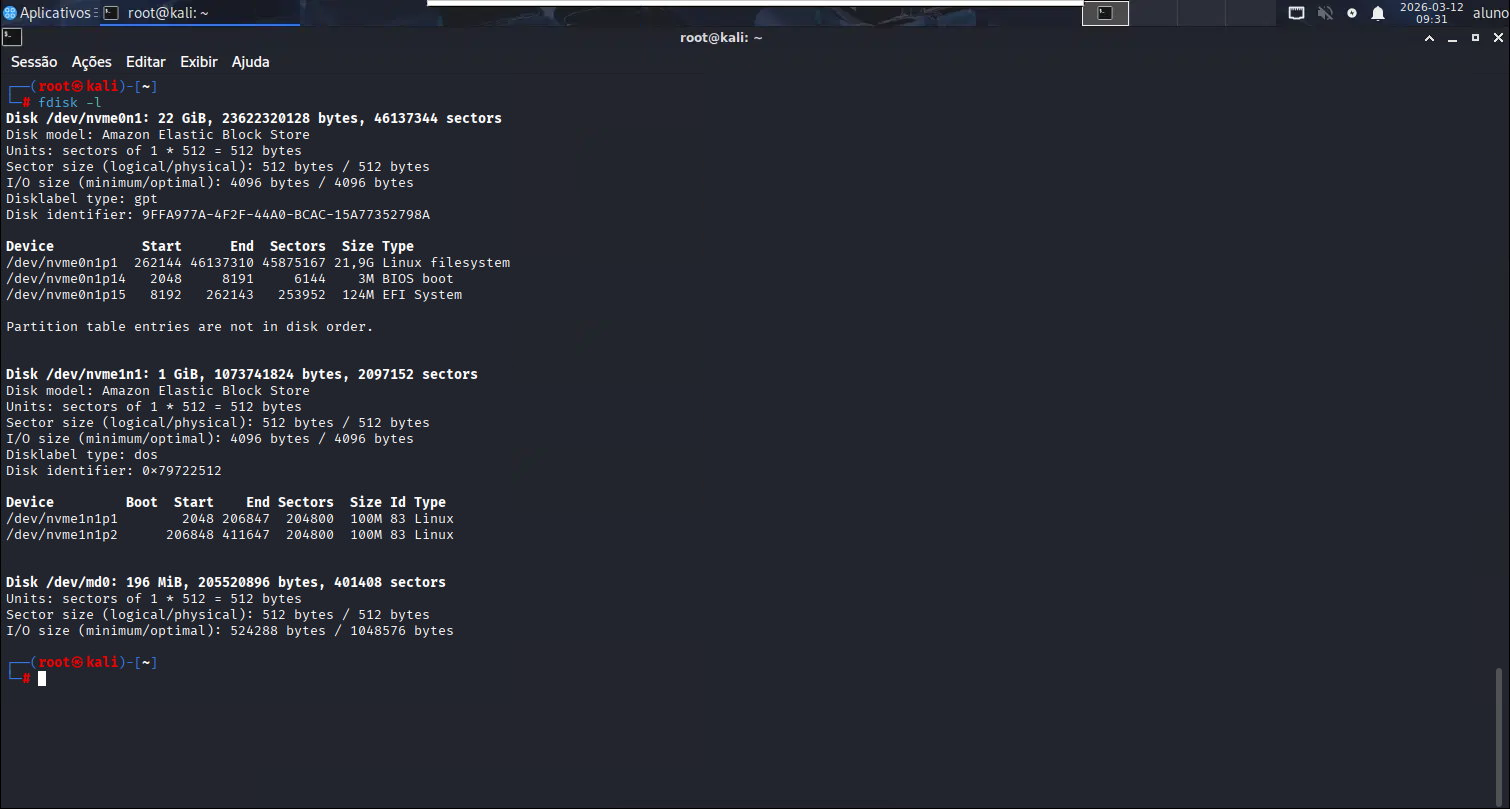
\includegraphics[width=0.99\textwidth]{./fig/fig7.1.png}
  \caption{Configuração de discos após criação do RAID 0 no Kali Linux}
  \label{fig:fig7.1}
\end{figure}

\newpage

\question[Atividade 7.2]{Aplicando o Software RAID 1 no Kali Linux}

\begin{figure}[H]
  \centering
  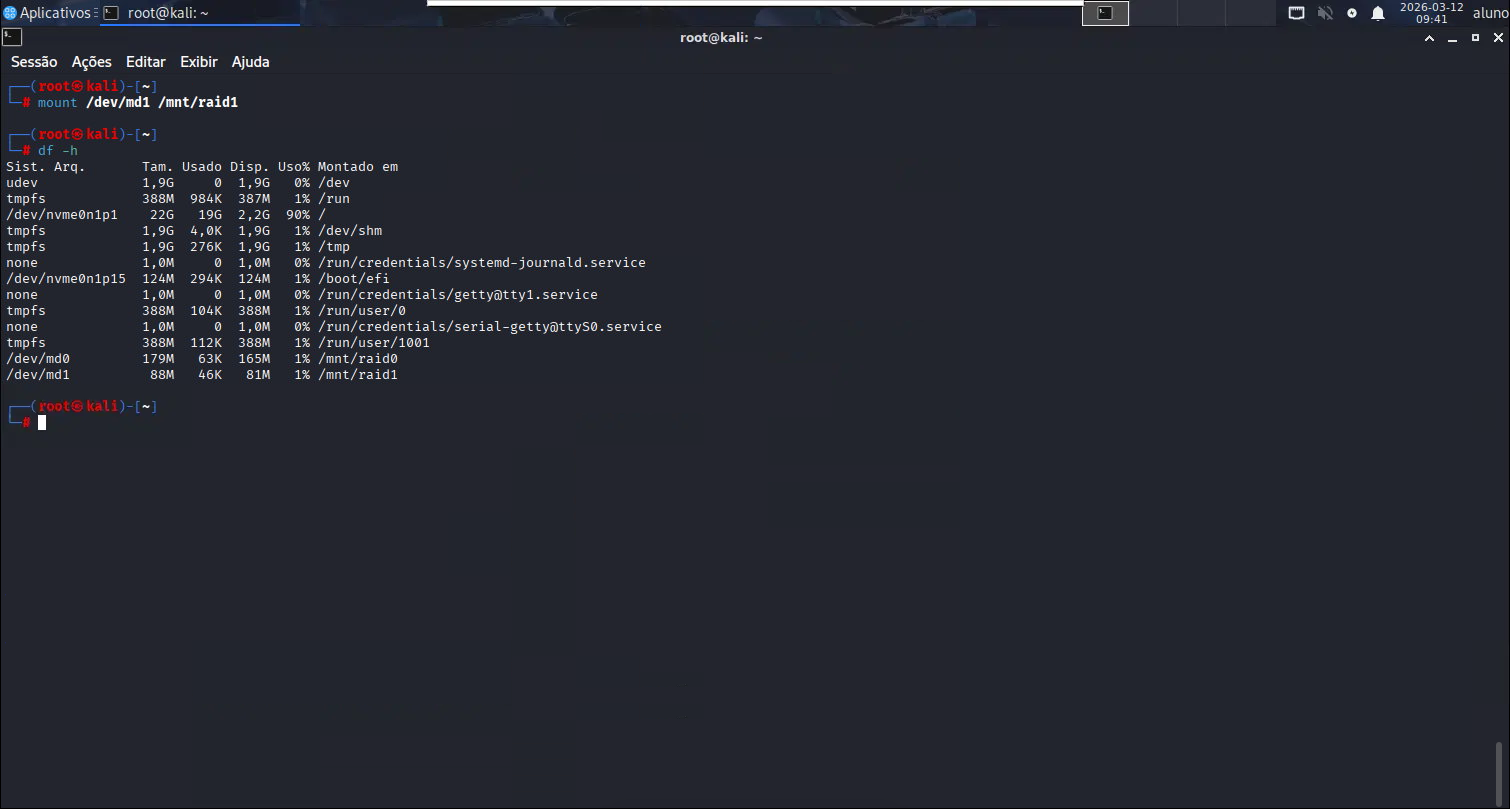
\includegraphics[width=0.99\textwidth]{./fig/fig7.2.png}
  \caption{Verificação do RAID 1 montado no diretório /mnt/raid1}
  \label{fig:fig7.2}
\end{figure}

\newpage

\question[Atividade 7.3]{Replicando conteúdo de pastas no Kali Linux com o Rsync de forma manual}

\begin{figure}[H]
  \centering
  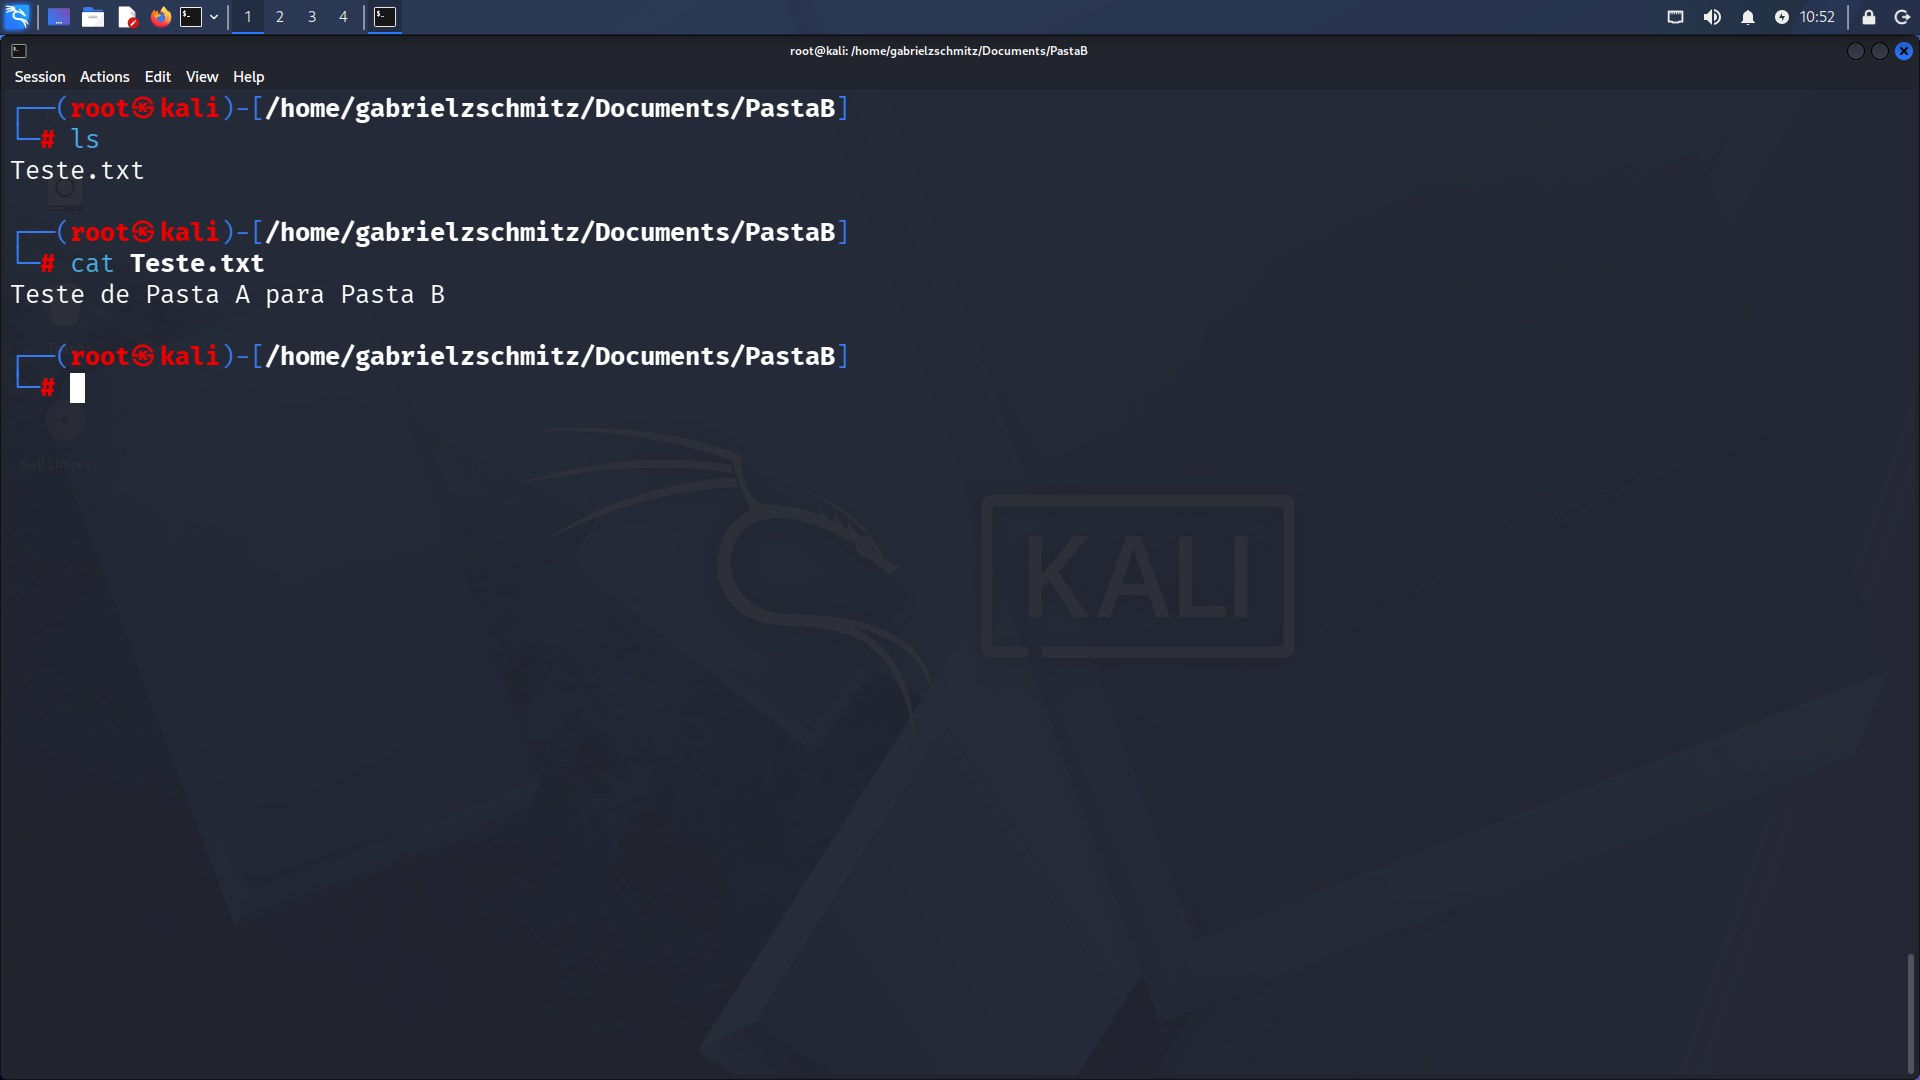
\includegraphics[width=0.99\textwidth]{./fig/fig7.3.png}
  \caption{Replicação manual do arquivo Teste.txt utilizando rsync}
  \label{fig:fig7.3}
\end{figure}

\newpage

\question[Atividade 7.4]{Replicando conteúdo de pastas automaticamente com Rsync}

\begin{figure}[H]
  \centering
  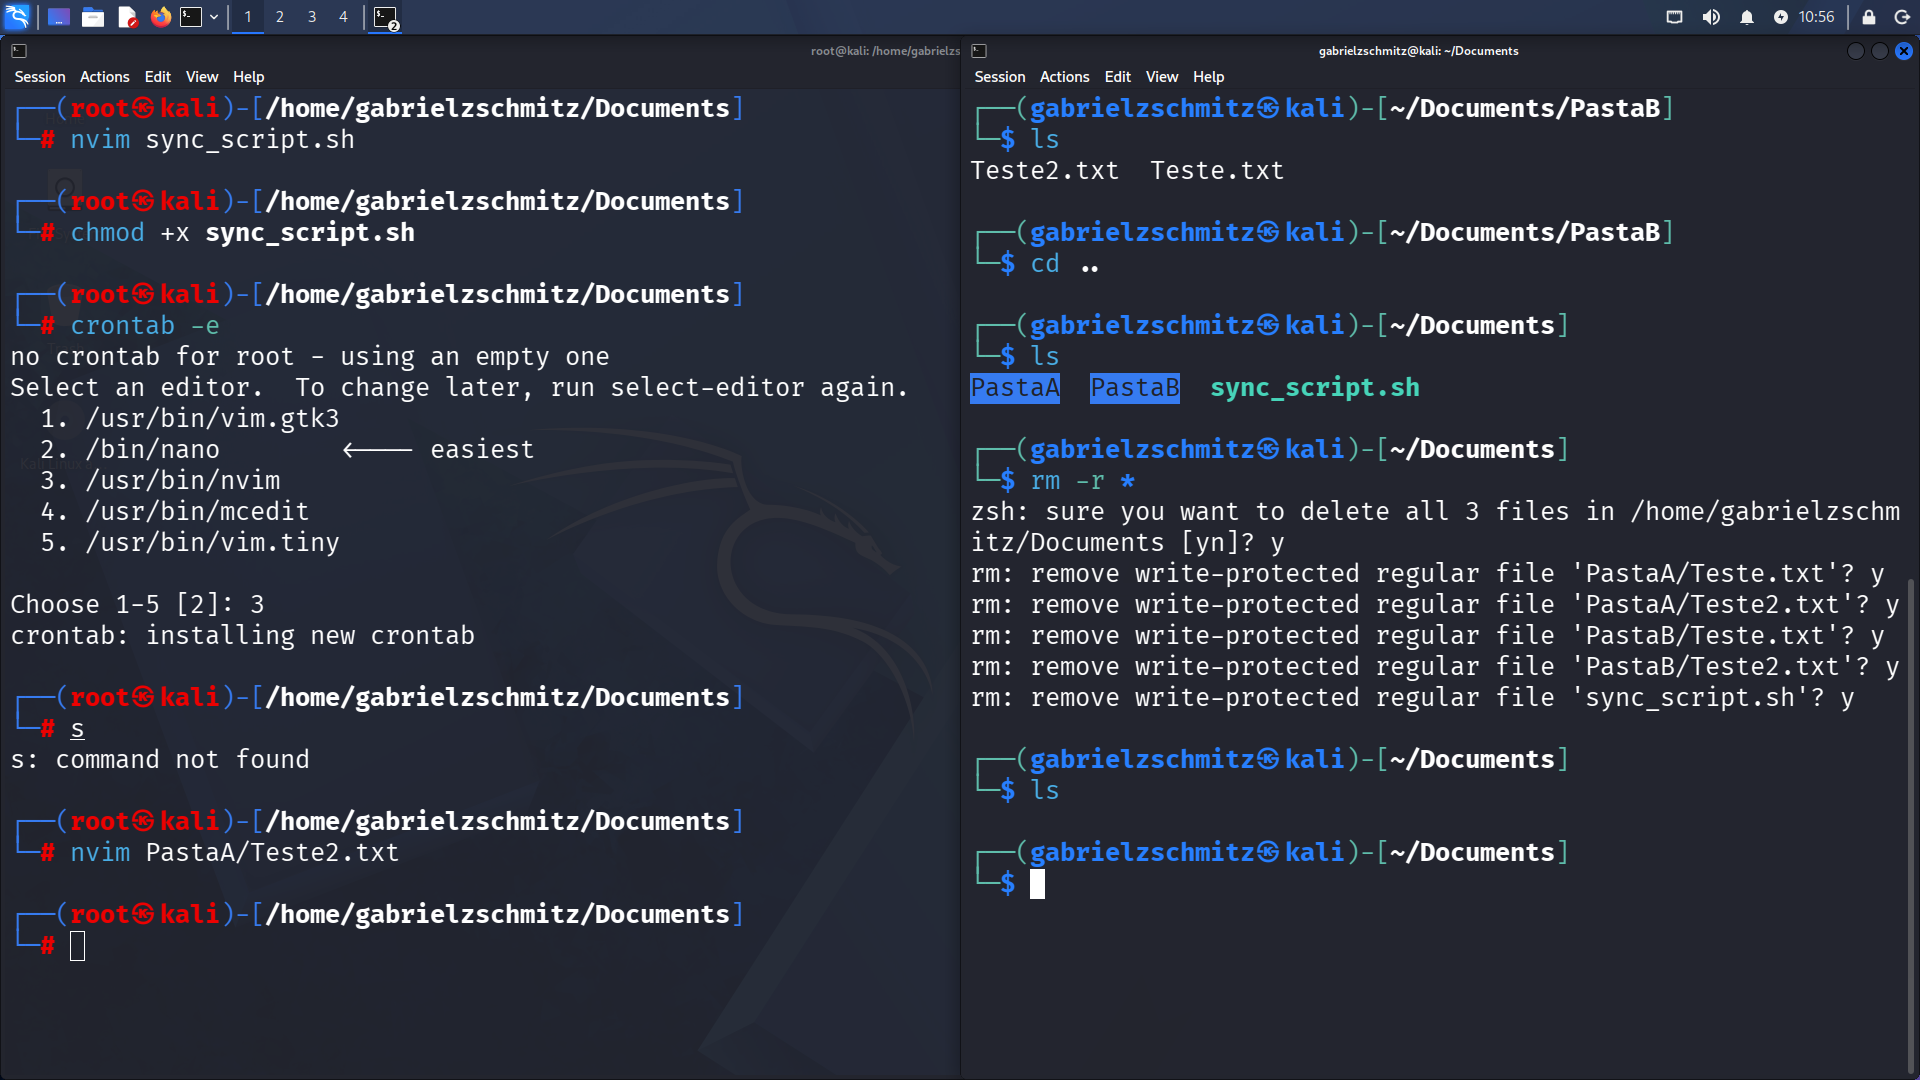
\includegraphics[width=0.99\textwidth]{./fig/fig7.4.png}
  \caption{Replicação automática de arquivos com rsync utilizando cron}
  \label{fig:fig7.4}
\end{figure}

\newpage

\question[Atividade 7.5]{Backup via replicação síncrona em nuvem no Windows Server 2022}

\begin{figure}[H]
  \centering
  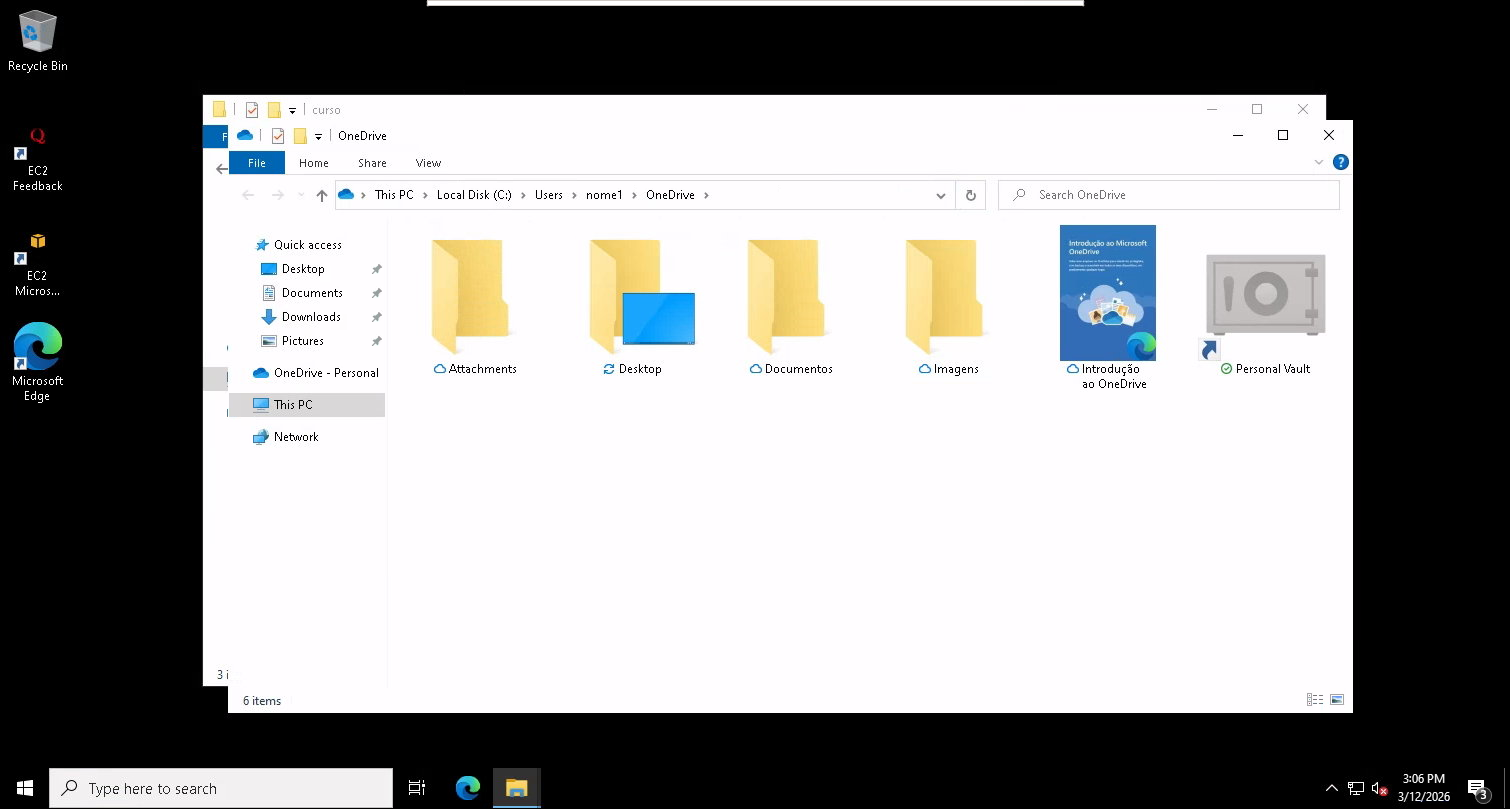
\includegraphics[width=0.99\textwidth]{./fig/fig7.5.png}
  \caption{Pasta do OneDrive sincronizada no Windows Server 2022}
  \label{fig:fig7.5}
\end{figure}
